% example.tex
\documentclass[dvisvgm]{standalone}

\usepackage{amsmath}
\usepackage[usenames,dvipsnames]{xcolor}
\usepackage{amsmath}
\usepackage{tikz}
\usetikzlibrary {arrows.meta,
                 positioning,
                 shapes.geometric}

 \tikzset{
        base/.style={draw, align=center, minimum height=4ex},
        proc/.style={base, rectangle, text width=8em},
        io/.style={trapezium, trapezium left angle=70, trapezium right
                   angle=110, draw, text width=8em, %minimum width=2cm, 
                   %minimum height=1cm
                   },
        test/.style={base, diamond, aspect=2,
                     %text width=5em
                     },
        term/.style={proc, rounded corners},
        myarrow/.style={-Stealth, line width=0.25mm},
 }

\begin{document}
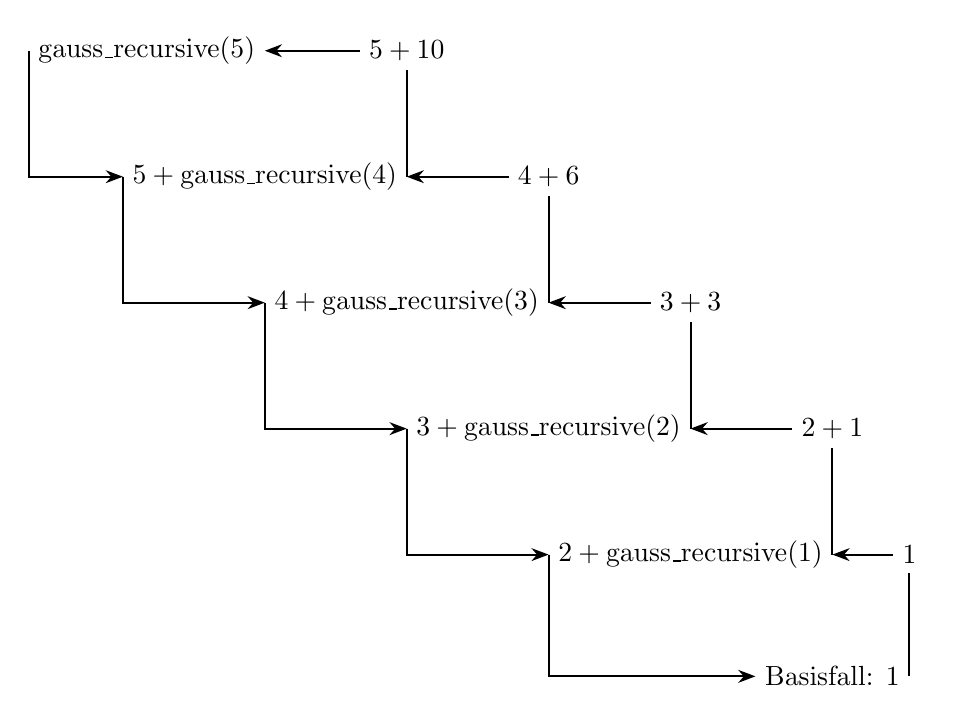
\begin{tikzpicture}
    \node (a) {gauss\_recursive(5)};
    \node[below=of a.south east] (b) {$ 5 + \text{gauss\_recursive(4)}$};
    \node[below=of b.south east] (c) {$ 4 + \text{gauss\_recursive(3)}$};
    \node[below=of c.south east] (d) {$ 3 + \text{gauss\_recursive(2)}$};
    \node[below=of d.south east] (e) {$ 2 + \text{gauss\_recursive(1)}$};
    \node[below=of e.south east] (f) {Basisfall: $1$};

    \draw[myarrow] (a.west) |- (b);
    \draw[myarrow] (b.west) |- (c);
    \draw[myarrow] (c.west) |- (d);
    \draw[myarrow] (d.west) |- (e);
    \draw[myarrow] (e.west) |- (f);

    \draw[myarrow] (f.east) |- node [fill=white] {$1$} (e.east);
    \draw[myarrow] (e.east) |- node [fill=white] {$2+1$} (d.east);
    \draw[myarrow] (d.east) |- node [fill=white] {$3+3$} (c.east);
    \draw[myarrow] (c.east) |- node [fill=white] {$4+6$} (b.east);
    \draw[myarrow] (b.east) |- node [fill=white] {$5+10$} (a.east);
\end{tikzpicture}
\end{document}
